\chapter{Preliminary analysis of \ac{AABW} samples}

\section{Introduction and Methods}
\begin{table}
\caption[\ac{AABW} samples used in the preliminary analysis]{Sampling time, location and physicochemical properties of \ac{AABW} samples used in this preliminary study.
All data were retrieved from the \ac{CTD} (SeaBird, Bellevue, USA) instrument used to collect the samples.}
\label{tab:deepsamples}
\smallskip
\begin{tabularx}{\textwidth}{llllXXXXXX}
\toprule
\textbf{Sample} & \textbf{Date} & \textbf{Latitude} & \textbf{Longitude} & \textbf{Sample Depth (m)} & \textbf{Temperature (\textdegree{}C)} & \textbf{Salinity (PSU)} & \textbf{Volume \linebreak filtered (L)}\\
\midrule

356 & 03/01/08 & $-66.7617$ & 144.4138 & 920 & $-1.9$ & 34.69 & 230\\
361 & 14/01/08 & $-66.4727$ & 140.5572 & 1170 & $-1.8$ & 34.56 & 225\\
365 & 23/01/08 & $-56.6967$ & 141.9125 & 3693 & 0.5 & 34.69 & 230\\
\bottomrule
\end{tabularx}
\end{table}

Three samples of \ac{AABW} were opportunistically obtained and analysed during the project described in \secreft{ch:polarfront}.
Two of these samples (356 and 361) were of newly formed \ac{AABW} waters on the Antarctic continental shelf, while one (365) was of abyssal \ac{AABW} from the South Australian basin \tabref{tab:deepsamples}.
DNA extraction, sequencing and construction of a taxonomic profile by \softwarename{blast} comparison to the RefSeq database were performed using the methods described in \secreft{ch:polarfront}.
A standardised and log-transformed Bray-Curtis resemblance matrix was constructed including the taxonomic profiles of the \ac{AABW} samples as well as the \ac{NZ} and \ac{SZ} samples described in \secreft{ch:polarfront}.
A \ac{nMDS} plot was then constructed from this matrix.
All statistical procedures were performed in \softwarename{PRIMER 6} as described by \citet{Clarke:2001ut}.

\section{Results and Discussion}

\begin{figure}
  \centering
  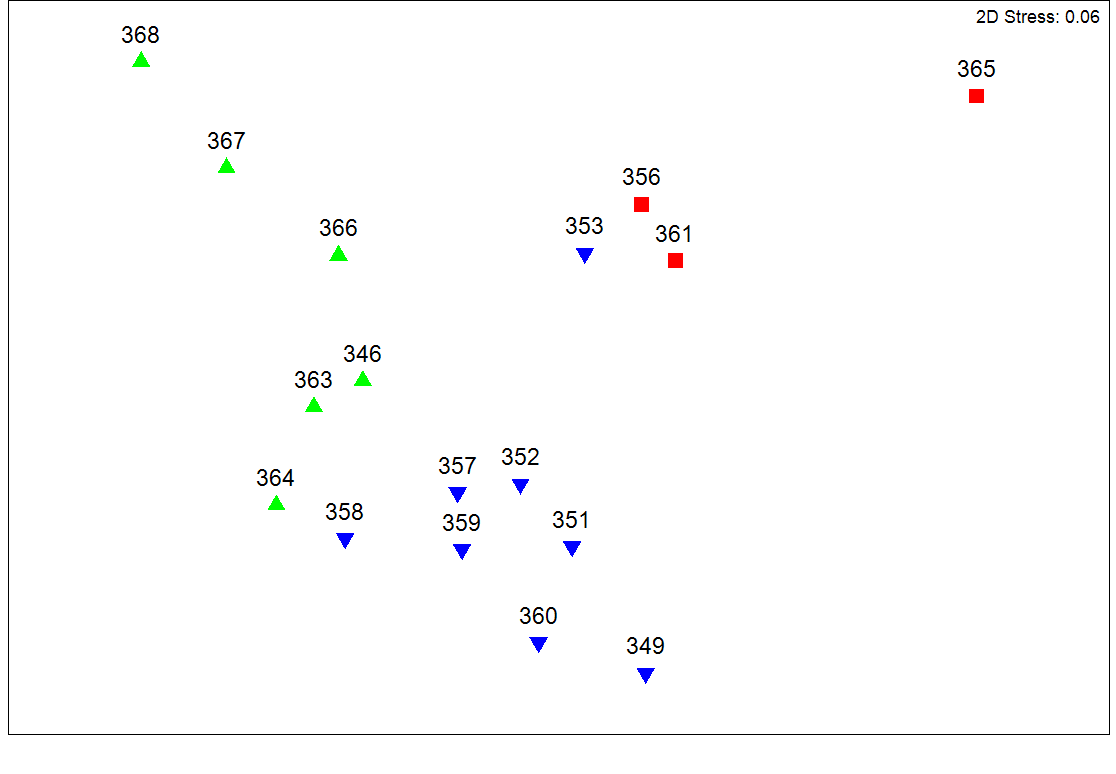
\includegraphics[width=\textwidth]{../biogeog/deepnmds.png}
  \caption[\ac{nMDS} of \ac{AABW}, \ac{NZ} and \ac{SZ} samples]{\ac{nMDS} plot showing distance between \ac{AABW}, \ac{NZ} and \ac{SZ} samples.
  Green triangles represent samples from the \ac{NZ}; blue inverted triangles from the \ac{SZ}; and red squares from \ac{AABW}.}
  \label{fig:deepnmds}
\end{figure}


Although the three \ac{AABW} samples were taken in deep, cold and aphotic waters \tabref{tab:deepsamples} compared to the surface \ac{AZ} and \ac{SZ} samples, the \ac{nMDS} plot suggested that the two continental shelf \ac{AABW} samples (356 and 361) were surprisingly similar to those of the \ac{AZ}, particularly sample 353 \figref{fig:deepnmds}.

\begin{sidewaystable}
\sffamily
\caption[Twenty most abundant \acp{OTU} in preliminary \ac{AABW} samples]{\sffamily{}Relative abundances (as percentages) of the twenty most abundant \acp{OTU} identified in the preliminary study of \ac{AABW} samples.}
\label{tab:topdeepotus}
\smallskip
\begin{tabularx}{\textheight}{Xlllllllll}
\toprule
\textbf{OTU} & \multicolumn{3}{c}{\textbf{Sample 356}} & \multicolumn{3}{c}{\textbf{Sample 365}} & \multicolumn{3}{c}{\textbf{Sample 361}}\\
\cmidrule(r){2-4}
\cmidrule(r){5-7}
\cmidrule(r){8-10}
& 0.1 \micron & 0.8 \micron & 3.0 \micron & 0.1 \micron & 0.8 \micron & 3.0 \micron & 0.1 \micron & 0.8 \micron & 3.0 \micron\\
\midrule
\candidatusfull{Pelagibacter ubique} HTCC1062 & 48.40 & 32.32 & 32.85 & 19.02 & 22.31 & 3.880 & 43.74 & 19.07 & 16.25\\
\speciesfull{Nitrosopumilus maritimus} SCM1 & 11.92 & 9.289 & 13.99 & 30.17 & 7.790 & 22.74 & 15.17 & 11.31 & 16.57\\
\candidatusfull{Ruthia magnifica} str. Cm (\species{Calyptogena magnifica}) & 3.780 & 4.563 & 2.356 & 2.844 & 1.504 & 0.2599 & 5.212 & 7.735 & 4.176\\
\candidatusfull{Vesicomyosocius okutanii} strain HA & 2.349 & 2.757 & 1.396 & 1.859 & 0.8025 & 0.08227 & 3.231 & 4.427 & 2.021\\
\genus{Roseobacter} sp. OCh114 & 0.1412 & 1.166 & 0.6845 & 0.08564 & 0.6662 & 0.4851 & 0.1509 & 1.853 & 0.8680\\
\candidatusfull{Puniceispirillum marinum} IMCC1322 & 0.3180 & 1.103 & 0.6403 & 0.4218 & 0.8223 & 0.4202 & 0.2878 & 1.259 & 0.5429\\
\species{Marinobacter hydrocarbonoclasticus} VT8 & 0.06999 & 0.4091 & 0.3976 & 0.2476 & 1.050 & 2.338 & 0.05732 & 0.5405 & 0.4616\\
\species{Silicibacter pomeroyi} DSS-3 & 0.1081 & 0.8406 & 0.4996 & 0.1290 & 0.4630 & 0.3621 & 0.1302 & 1.522 & 0.6347\\
\species{Robiginitalea biformata} strain HTCC2501 & 0.2813 & 0.6433 & 0.7417 & 0.1769 & 0.2739 & 0.4978 & 0.2213 & 0.9391 & 0.8442\\
\species{Pseudoalteromonas haloplanktis} strain TAC125 & 0.02530 & 0.4540 & 0.1958 & 0.2836 & 2.817 & 0 & 0.01876 & 0.3389 & 0.2552\\
\species{Alcanivorax borkumensis} strain SK2 & 0.09262 & 0.3163 & 0.4281 & 0.1049 & 0.5674 & 1.985 & 0.04843 & 0.3412 & 0.3920\\
\species{Gramella forsetii} strain KT0803 & 0.3096 & 0.6465 & 0.7405 & 0.1254 & 0.2670 & 0 & 0.1883 & 0.9402 & 0.8114\\
\genus{Colwellia} sp. 34H & 0.04289 & 0.4512 & 1.020 & 0.07200 & 0.4532 & 0.7727 & 0.03922 & 0.5015 & 0.6107\\
\species{Flavobacterium psychrophilum} strain JIP02/86 & 0.2417 & 0.4722 & 0.6353 & 0.07943 & 0.1645 & 0.5072 & 0.1587 & 0.7866 & 0.6579\\
\species{Pirellula staleyi} strain DSM 6068 & 0.003149 & 0.2477 & 0.3093 & 0.08767 & 1.401 & 0.7732 & 0.003149 & 0.2410 & 0.3146\\
\genus{Jannaschia} sp. DFL-12 & 0.07995 & 0.6770 & 0.3841 & 0.03865 & 0.2030 & 0.1025 & 0.1015 & 1.075 & 0.4369\\
\species{Pseudoalteromonas atlantica} strain T6c & 0.02312 & 0.1653 & 0.1941 & 0.03856 & 0.3235 & 1.728 & 0.01733 & 0.1541 & 0.3157\\
\species{Zunongwangia profunda} strain SM-A87 & 0.1830 & 0.3499 & 0.4826 & 0.1036 & 0.1362 & 0.3825 & 0.1193 & 0.5573 & 0.6261\\
\genus{Silicibacter} sp. TM1040 & 0.09568 & 0.5448 & 0.3455 & 0.03477 & 0.2014 & 0.1740 & 0.09949 & 1.021 & 0.3676\\
\species{Capnocytophaga ochracea} strain DSM 7271 & 0.1251 & 0.2916 & 0.4491 & 0.03893 & 0.1542 & 0.5332 & 0.1049 & 0.4062 & 0.5307\\
\bottomrule
\end{tabularx}
\end{sidewaystable}

